\chapter{Evaluation}
\label{chap:evaluation}
We conducted three experiments to evaluate the performance of our implementation: two focused on throughput and one on latency.
The first experiment examines throughput based on the packet size, while the second assesses throughput in relation to the number of filter rules in a netfilter-based application.
The third experiment investigates the latency associated with different packet forwarding mechanisms.


We compare the performance of \texttt{End.AN.NF} with three forwarding mechanisms: \texttt{End}, the combination of \texttt{End.DT4} and \texttt{H.Encaps}, and IPv4, which serves as a baseline.
As shown in Figure 1, when \texttt{End.AN.NF} operates, a received packet passes through twice the number of hook points compared to \texttt{End}.
Hence, the performance of \texttt{End.AN.NF} might be inferior to \texttt{End}.
On the other hand, the performance of \texttt{End.AN.NF} is expected to be higher than the combination of \texttt{End.DT4} and \texttt{H.Encaps}.
When applying netfilter rules to packets encapsulated in SRv6, a practical approach in a vanilla Linux kernel is the combination of \texttt{End.DT4} and \texttt{H.Encaps}.
Vanilla Linux kernel does not have a method to apply netfilter to a packet that is still encapsulated in SRv6.
Therefore, it needs to decapsulate the packet once and encapsulate it instead of the originally attached SRH again.
A packet decapsulated by \texttt{End.DT4} passes through netfilter hook points as an IPv4 packet, and \texttt{H.Encaps} stores new SRH.
Thus, this method has overheads because it requires \texttt{End.DT4} to decapsulate the packet and then \texttt{H.Encaps} to encapsulate the packet again.
Therefore, it is anticipated that this overhead will lead to a degradation in performance.


%Hence: したがって,それ故に
%
% なんのために評価をするのかはじめに書く
% この研究で何を評価するのか,比較するのかを書く
% 目的: \texttt{End.AN.NF} のパフォーマンスを調べること
% それぞれ 3 つのパフォーマンスを調べた.
% その比較対象として, ただの End と End.DT..., IPv4 を比較対象として上げる.
% この部分で End.DT... の話をする
% 良かったのかわるかったのかは比較するひつようがある
% それぞれが何かはここで説明する
% 「なぜそれらと比較するのか」 を書く
% IPv4 はベースラインである. そもそも SRv6 の転送が遅いのでは? という読者の疑問に対して示す.
% End.DT... との比較: 既存の手法と比べてオーバーヘッドが減っているはずだよね. ということを示す
% End.DT... はオーバヘッドがありそう, End よりは遅そう などの予想を書いておく. 実際の結果を順番に示していく.
% the combination of \texttt{End.DT4}6 and \texttt{H.Encaps} would involve overhead compared with \texttt{End.AN.NF}. 的な
% 読者が順番に読んで疑問を持たないですっと読めるようにする.

% ちゃんと構成するには初稿を上げたのと同じくらい時間がかかるので,とにかく埋める.

The environment is the same configuration for all experiments.
We prepared two machines directly connected with a 100 Gbps link.
The two machines are identical: Intel(R) Xeon(R) Silver 4310 12-core CPU x2, 64-GB DDR4-2666 memory, and Intel E810 100 Gbps NIC.
We disabled The CPU's hyperthreading function.
One is used as a traffic generator, and the other as a System Under Test (SUT).
In the traffic generator machine, we installed Ubuntu 22.04 and TRex~\cite{trex}, which we used to generate test traffic.
In the SUT machine, we installed the customized Linux kernel 5.15.106, where we have implemented \texttt{End.AN.NF} and the customized iproute2 command to configure \texttt{End.AN.NF} SIDs.
We also prepared two VLANs on the link between the two machines.


\subsection{Throughput per packet size}
\label{ssec:eval.thru-size}

We measured the throughput of \texttt{End.AN.NF}, \texttt{End}, IPv4, and the combination of \texttt{End.DT4} and \texttt{H.Encaps} while changing the packet size to increase.
This experiment clarifies the change in throughput with packet size for each packet forwarding mechanism.
We did not use any netfilter rules in this experiment.
We assessed the throughput reduction of \texttt{End.AN.NF} in comparison to \texttt{End} and the performance improvement of \texttt{End.AN.NF} over the combination of \texttt{End.DT4} and \texttt{H.Encaps}.


We sent traffic generated by TRex on the traffic generator machine to the SUT machine, from a minimum packet length of 126 bytes to a maximum packet length of 1518 bytes.
We calculated the packet length at the time of measurement as follows: $l=174n+126$.
$l$ means the length of the packet, and $n$ means the number of measurements.
We collected a total of 10 measurements, from $n=0$ to $n=10$.


The reason we chose a packet length of 126 bytes as a minimum packet length is the minimum length for a UDP packet with a tagged VLAN when the SID list length is two.
\texttt{End.AN.NF} mandates a SID list length of at least two, as it decrements the packet's segleft, which must remain zero or above.
With a SID list length of one, the segleft starts at zero, and decrementing it with \texttt{End.AN.NF} would result in a negative value.
Conversely, \texttt{End.DT4} necessitates that the segleft is zero.
In the measurement of the combination of \texttt{End.DT4} and \texttt{H.Encaps}, TRex generated packets with a SID list length of two but set the segleft to zero.
To effectively use the Receive Side Scheduling (RSS) mechanism, TRex incremented both the destination and source addresses of the inner IPv4 packet during packet generation.
For IPv4, we embedded dummy data in the UDP payload to match the SRv6 packet length, starting the packet length at 126 bytes.
We also incremented the destination and source addresses during packet generation to leverage RSS effectively.
Given that the maximum size of an Ether frame, including the tagged VLAN header, is 1518 bytes, we set the upper packet size limit to 1518 bytes for this measurement.


Figure~\ref{fig:size-thru} shows the result of this experiment.
The throughput of \texttt{End.AN.NF} never degrades by more than 6\% compared to \texttt{End} across all packet lengths.
For a packet length of 1518 bytes, \texttt{End.AN.NF} exhibits the least throughput degradation relative to \texttt{End}, approximately 1.7\%.
Conversely, about 5.6\% of the highest degradation occurs at a packet length of 478 bytes when comparing \texttt{End.AN.NF} to \texttt{End}.
There is no correlation between packet length and throughput, which varied significantly.
This degradation in throughput can be attributed to packets in \texttt{End.AN.NF} traversing twice the number of netfilter hook points compared to those in \texttt{End}, which remains within an acceptable range.


When comparing the throughput of \texttt{End.AN.NF} to the combination of \texttt{End.DT4} and \texttt{H.Encaps}, \texttt{End.AN.NF} consistently outperforms, irrespective of the packet length, as anticipated.
Specifically, \texttt{End.AN.NF} achieves a throughput that is 26.7\% higher than that of the \texttt{End.DT4} and \texttt{H.Encaps} combination.
The throughput disparity between \texttt{End.AN.NF} and the combination of \texttt{End.DT4} and \texttt{H.Encaps} is influenced by packet length: shorter packets result in a larger relative performance gap, while longer packets yield a narrower difference.
The packet per second (pps) rate increases as packet size decreases.
As a result, smaller packet sizes make any overheads in packet forwarding more noticeable.


\begin{figure}[t]
  \centering
  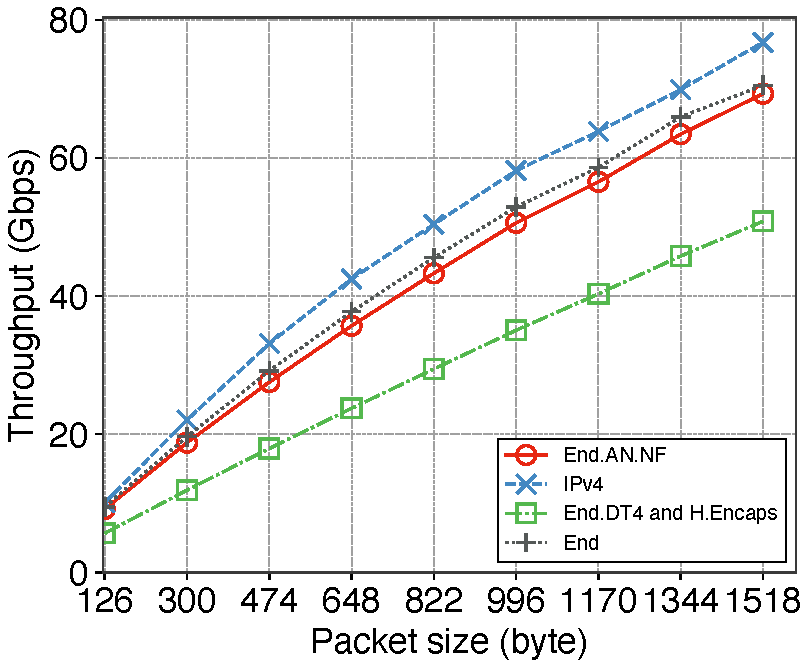
\includegraphics[width=0.95\linewidth]{img/size-throughput.pdf}
  \caption{Throughput per SRv6 End behaviors and IPv4}
  \label{fig:size-thru}
\end{figure}


\subsection{Throughput per number of filter rules installed in netfilter}
\label{ssec:eval.thru-chains}

Next, we evaluated the throughput of \texttt{End.AN.NF}, IPv4, and the combination of \texttt{End.DT4} and \texttt{H.Encaps}, varying the number of filter rules installed in netfilter.
We used nftables as a netfilter-based application to install filter rules.
In nftables, the rules are expressed as sets of chains.
There are two types of chains: base chains and regular chains.
All filter rules in base chains apply to forwarding packets.
nftables uses the regular chains only when the other chain refers to the regular chain.
In our experiment, we gauged the throughput for each chain type, incrementing the count of each chain type.
We anticipated a throughput decline with the addition of filter rules, irrespective of the forwarding mechanisms.
This experiment aims to clarify the characteristic of the throughput degradation for each packet forwarding mechanism due to the filter rules.


We sent traffic generated by TRex on the traffic generator machine to the SUT machine.
For this measurement, we set the packet length consistently at 126 bytes.
Our choice for a 126-byte packet length aligns with the rationale provided in Section~\ref{ssec:eval.thru-size}, which corresponds to the minimum length of a UDP packet with a tagged VLAN when the SID list length is two.


Figure~\ref{fig:rule-thru} illustrates the throughput per number of rules of base chains.
The chain rule is one of the worst cases of the nftables chain rule.
In this measurement, we installed filter rules at the netfilter's forward hook point.
These rules are consistently designed to accept all passing packets and then apply the same subsequent rule.
netfilter permits the installation of multiple rules on a single hook point.
Throughout the experiment, we incrementally increased the number of these identical cascading rules applied at this hook point.
Across all packet-forwarding mechanisms, throughput diminishes with an increasing number of rules.
As rule count rises, the throughput for all three mechanisms converges to approximately 0.4 Mbps.
When comparing the throughput of \texttt{End.AN.NF} and IPv4, there is no pronounced disparity of characteristics in throughput decline, with \texttt{End.AN.NF} not showing any significant disadvantage relative to IPv4.
Consistently, \texttt{End.AN.NF} outperforms the combination of \texttt{End.DT4} and \texttt{H.Encaps} in terms of throughput.
However, this performance gap narrows with increasing rule count, reaching a mere 9\% difference at 128 rules.
As the rule count in the regular chain escalates, the advantage of \texttt{End.AN.NF} over the combination of \texttt{End.DT4} and \texttt{H.Encaps} diminishes.


Figure~\ref{fig:reg-thru} presents the throughput as per number of rules in regular chains.
Notably, there's no observed degradation in throughput, \texttt{End.AN.NF} consistently outperforms the combination of \texttt{End.DT4} and \texttt{H.Encaps}.
The filter rules for regular chains were the same configuration as when we measured for the base chains, consistently designed to accept all passing packets and then apply the same subsequent rule.
However, in this chain rule configuration, none of the defined regular chains are referenced by other chains, so none of the rules configured in regular chains apply to the packets.
As a result, the actual number of rules applied as packets traverse the netfilter hook point remains unchanged.

\begin{figure}[t]
  \centering
  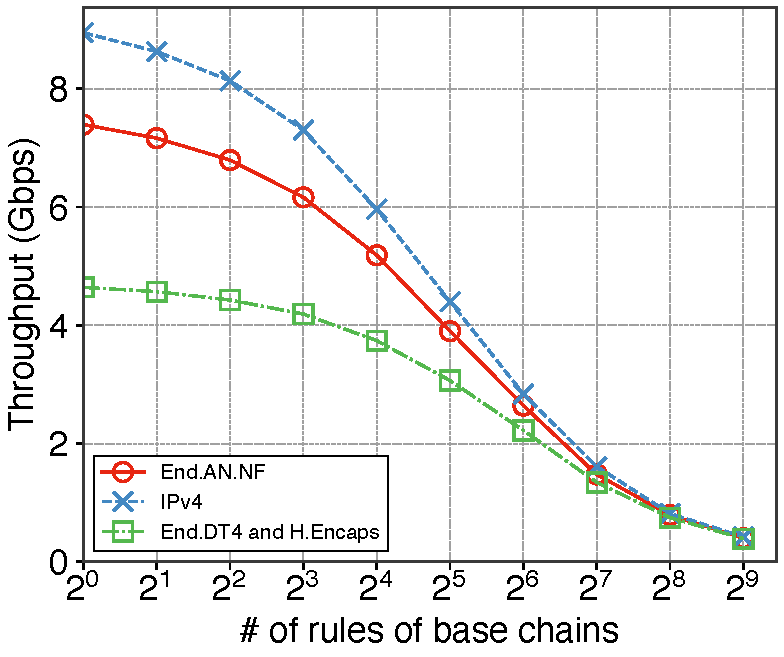
\includegraphics[width=0.95\linewidth]{img/rule-throughput.pdf}
  \caption{Throughput per number of rules of base chains}
  \label{fig:rule-thru}
\end{figure}

\begin{figure}[t]
  \centering
  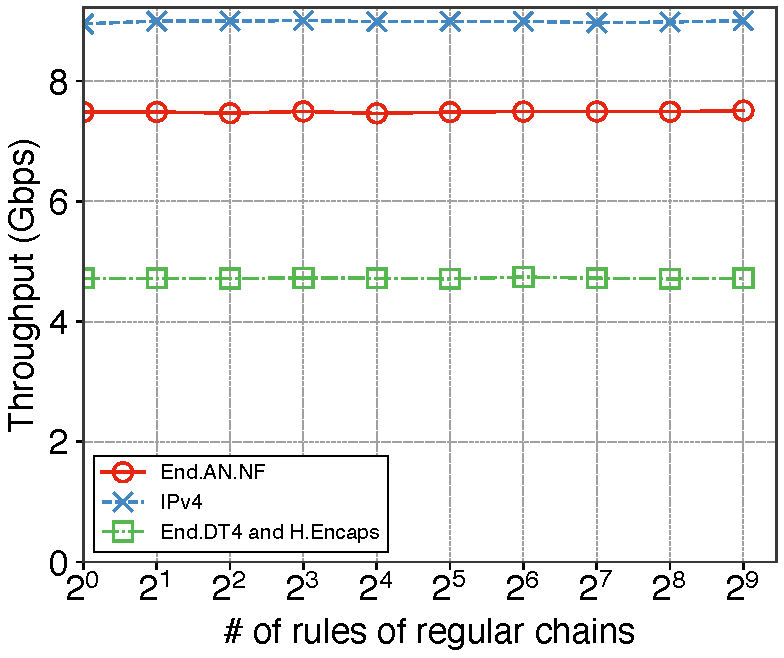
\includegraphics[width=0.95\linewidth]{img/regular-throughput.pdf}
  \caption{Throughput per number of rules of regular chains}
  \label{fig:reg-thru}
\end{figure}

\subsection{Latency of End.AN.NF, End, IPv4, and the combination of End.DT4 and H.Encaps}
\label{ssec:eval.rtt}
% 全体的に短すぎるが,単純すぎて書くことが思いつかない.


We also measured the latency of \texttt{End.AN.NF}, \texttt{End}, IPv4, and the combination of \texttt{End.DT4} and \texttt{H.Encaps}.
This experiment focused on latency.
Our objective was to evaluate the latency of \texttt{End.AN.NF} by comparing its degradation relative to \texttt{End} and its improvement when juxtaposed with the combination of \texttt{End.DT4} and \texttt{H.Encaps}.
For this evaluation, we used IPv4 latency as the baseline reference.


We measured packet forwarding latency using TRex.
TRex can capture the time interval between packet transmission and reception in microsecond resolution.
In this measurement, the packet length was 142 bytes: 126 bytes is the minimum packet length \texttt{End.AN.NF} requires, as explained in Section~\ref{ssec:eval.thru-size}, and the next 16 bytes is used to pass information needed to measure latency by TRex.
During the experiment, the traffic generator dispatched 10000 packets per second to the SUT for 10 seconds.
We disabled RSS in this measurement by not changing the source and destination addresses.
At this level of pps, distributing CPU cores using RSS would worsen latencies and cause extra jitter.


The result is shown in Figure~\ref{fig:rtt}.
Each data point on these graphs represents the average of 100,000 latency measurements.
The latencies for \texttt{End.AN.NF}, \texttt{End}, and IPv4 are consistently 16.0 microseconds.
In contrast, the combination of \texttt{End.DT4} and \texttt{H.Encaps} exhibits a latency of 19.0 microseconds.
When measured in microsecond resolution, \texttt{End.AN.NF} matches the latency of \texttt{End} and IPv4 and is approximately 15.8\% faster than the \texttt{End.DT4} and \texttt{H.Encaps} combination.

\begin{figure}[t]
  \centering
  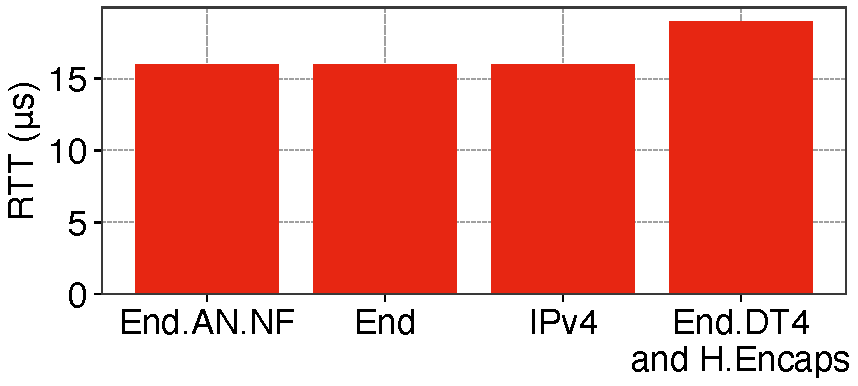
\includegraphics[width=0.95\linewidth]{img/latency.pdf}
  \caption{Latency per SRv6 End behaviors and IPv4}
  \label{fig:rtt}
\end{figure}